\documentclass[11pt]{article}
\pdfinfoomitdate=1\pdftrailerid{}
\usepackage[letterpaper,margin=.7in,headheight=15pt,headsep=18pt,footskip=24pt]{geometry}
\usepackage[T1]{fontenc}
\usepackage{lmodern,amsmath,amssymb,array,booktabs,fancyhdr,tikz,hyperref}
\renewcommand{\familydefault}{\sfdefault}
\setlength{\parindent}{0pt}\setlength{\parskip}{6pt}
\pagestyle{fancy}\fancyhf{}
\fancyhead[L]{\small Week 58 / Fair division / Adult return-visit guide}
\fancyfoot[L]{\scriptsize Bellingham Math Circle / Week 58 / W58-RV-FAC-v2}
\fancyfoot[R]{\thepage}
\newcommand{\head}[1]{\par\textbf{\large #1}\par}
\newcommand{\sub}[1]{\par\textbf{#1}\par}
\newcommand{\hint}[1]{\textit{If needed:} #1}
\newcommand{\seq}[1]{\texttt{#1}}
\hypersetup{hidelinks}
% Generated and rechecked by check_guide.py; do not edit by hand.
\newcommand{\ktable}{%
\begin{tabular}{@{}rll@{}}
\textbf{Row} & \textbf{Train with minimum cuts} & \textbf{Fewest}\\\midrule
1 & \texttt{RB|RB} & 1\\
2 & \texttt{R|RB|B} & 2\\
3 & \texttt{BR|RB} & 1\\
4 & \texttt{B|BR|R} & 2\\
5 & \texttt{RB|BR} & 1\\
6 & \texttt{BR|BR} & 1\\
\end{tabular}}
\newcommand{\ksecond}{%
\begin{tabular}{@{}rll@{}}
\textbf{Row} & \textbf{Train with minimum cuts} & \textbf{Fewest}\\\midrule
1 & \texttt{RR|RRB|B} & 2\\
2 & \texttt{BRR|BRR} & 1\\
3 & \texttt{RBRBR} & impossible\\
4 & \texttt{RRBB|BBRR} & 1\\
5 & \texttt{RR|RRBB|BB} & 2\\
6 & \texttt{RRRBB|BBRRR} & 1\\
7 & \texttt{RRR|RRRBB|BB} & 2\\
\end{tabular}}
\newcommand{\msecond}{%
\begin{tabular}{@{}rll@{}}
\textbf{Row} & \textbf{Train with minimum cuts} & \textbf{Fewest}\\\midrule
1 & \texttt{RR|RRB|B} & 2\\
2 & \texttt{RB|BRR|R} & 2\\
3 & \texttt{BRRB|RRBB} & 1\\
4 & \texttt{R|RRBB|BBR} & 2\\
5 & \texttt{RBRRBRB} & impossible\\
6 & \texttt{RR|BRRRB|BBR} & 2\\
7 & \texttt{RBBRR|RRBBR} & 1\\
\end{tabular}}
\newcommand{\utable}{%
\begin{tabular}{@{}rll@{}}
\textbf{Row} & \textbf{Train with minimum cuts} & \textbf{Fewest}\\\midrule
1 & \texttt{R|RRBB|BBR} & 2\\
2 & \texttt{BRRB|RBBR} & 1\\
3 & \texttt{RR|RRBB|BB} & 2\\
4 & \texttt{RBRR|RRBRB|B} & 2\\
5 & \texttt{BBRRR|RRRBB} & 1\\
6 & \texttt{RRR|RRRB|B} & 2\\
\end{tabular}}
\newcommand{\allfour}{%
\begin{tabular}{@{}lll@{}}
\textbf{Train} & \textbf{Cuts} & \textbf{Fewest}\\\midrule
\texttt{BBRR} & \texttt{B|BR|R} & 2\\
\texttt{BRBR} & \texttt{BR|BR} & 1\\
\texttt{BRRB} & \texttt{BR|RB} & 1\\
\texttt{RBBR} & \texttt{RB|BR} & 1\\
\texttt{RBRB} & \texttt{RB|RB} & 1\\
\texttt{RRBB} & \texttt{R|RB|B} & 2\\
\end{tabular}}
\newcommand{\gametable}{%
\begin{tabular}{@{}lllll@{}}
\textbf{Order} & \textbf{First marks A B C} & \textbf{First taker} & \textbf{Second marks} & \textbf{Second taker}\\\midrule
X Y Z & 50, 100, 25 & C at 25 & A: 62.5, B: 100 & A at 62.5\\
X Z Y & 50, 75, 25 & C at 25 & A: 112.5, B: 75 & B at 75\\
Y X Z & 25, 50, 75 & A at 25 & B: 112.5, C: 75 & C at 75\\
Y Z X & 25, 50, 100 & A at 25 & B: 62.5, C: 100 & B at 62.5\\
Z X Y & 100, 25, 50 & B at 25 & A: 100, C: 62.5 & C at 62.5\\
Z Y X & 75, 25, 50 & B at 25 & A: 75, C: 112.5 & A at 75\\
\end{tabular}}
\newcommand{\scoretable}{%
\begin{tabular}{@{}lllll@{}}
\textbf{Order} & \textbf{A sees A B C} & \textbf{B sees A B C} & \textbf{C sees A B C} & \textbf{Envy}\\\midrule
X Y Z & 4, 6, 2 & 1, 11, 0 & 4, 4, 4 & A to B\\
X Z Y & 8, 2, 2 & 8, 4, 0 & 2, 6, 4 & B to A, C to B\\
Y X Z & 4, 2, 6 & 2, 8, 2 & 0, 8, 4 & A to C, C to B\\
Y Z X & 4, 4, 4 & 2, 4, 6 & 0, 1, 11 & B to C\\
Z X Y & 11, 0, 1 & 4, 4, 4 & 6, 2, 4 & C to A\\
Z Y X & 4, 0, 8 & 6, 4, 2 & 2, 2, 8 & A to C, B to A\\
\end{tabular}}

\begin{document}
\head{Mathematical overview}
\textbf{Two colours need at most two cuts.} Even counts of reds and blues can be shared equally into two trays using at most two gaps. Cards stay whole and pieces keep their order; a tray may receive several pieces. An odd colour count makes sharing impossible.

\textbf{Proof by a moving window.} Write the counts as $2r$ reds and $2b$ blues. Move a window of $r+b$ cards from the left end to the right. Its red count goes from $q$ to $2r-q$ (the end windows partition the train), changing by at most one per step. It reaches $r$, with $b$ blues. Give that window to one tray and the ends to the other: at most two gaps. One gap works exactly when the first half holds half of each colour.

\textbf{Two continuous tastes also need at most two cuts.} Assume nonnegative additive values with no value stuck at a point. Slide a half-value window for A from the left end to the right, keeping A's value fixed. Its final piece complements its initial piece, so B's value passes through half. Cut out the window and put the ends together. For zero-valued stretches, approximate by positive densities and take limits of the two endpoints. This continuous counterpart of the train proof is not a page task.

\textbf{Exact halves for all observers.} Half of each colour gives half the value to every taste uniform within that colour, including zero prices. The printed opposite tastes force these fractions, needing two cuts. On X, Y, Z, adding the three equal-value equations and comparing them forces half of every panel, needing three cuts. As literature background, $k$ nonatomic tastes (or $k$ even-count colours) admit exact bisection with at most $k$ cuts (Hobby--Rice; necklace splitting). This theorem is not proved here; X, Y, Z attains its three-taste bound.

\textbf{The marking game guarantees a third, not freedom from envy.} With fixed nonnegative additive values accumulating continuously, let $T_i$ be person $i$'s original total. Each remaining person marks a prefix worth $T_i/3$ from the new left end. The leftmost marker takes that prefix: exactly their third. Each removed prefix was worth at most $T_i/3$ to anyone waiting, leaving the last person at least $T_i-2T_i/3=T_i/3$. Enough remains for every mark; break ties either way. Here $T_i=12$: always target 4, \emph{not a third of the remainder}.

\textbf{Only two cards can be split.} There are two selected cut locations in a three-person marking game on a row of cards. Each cuts at most one card; a gap cuts none. This bound can be necessary. The general $n$-person version targets $T_i/n$ and uses at most $n-1$ cut locations, under the same divisible-value assumptions.

\textbf{Discoveries and demands.} K--1 experiments show that unmatched halves can still be shared by taking a middle piece; ``none needs three gaps'' may become a shared conjecture. Grades 2--3 checks the one-cut criterion, conjectures the two-cut bound, finds exact strip halves, and sees a guaranteed third coexist with envy. Grades 4--5 explains the window, proves the three-panel obstruction and marking guarantee, and bounds split cards. Finite examples suggest a rule; complete small catalogues or arguments establish it.

Adults read rules and the marking-game paragraph. K--1 counts to six; adults may scribe children's built trains. Grades 2--3 uses millimetres, halves and a quarter-panel mark. Grades 4--5 uses fractions and fixes one observer across three trays. Physical cuts approximate exact lengths.
\newpage
\head{Preparation and a manageable hour}
\textbf{Status.} Unpiloted and physically unrehearsed. Print scale, tray fit, handling ten-card trains, cutting at marked points, quarter-panel marks, staffing and timings have not been tested with this return visit.

\textbf{Reuse the base kit.} Follow W58-guide-v4, p. 3: five pair kits (two at K--1, two at grades 2--3, one at grades 4--5) and the three-person kit. Print W58-materials-v3 single-sided on Letter at Actual Size; pages 2--8 landscape. Check its 100 mm bars and cut outside borders. Trains are built on the table, not on the schematic records.

\textbf{Per pair.} Base goods plus an extra unmounted materials p. 1 gives six reds/four blues; set the spare paper R3 aside. Use two 150--180 mm trays, ruler, pencils, crayons and scrap; allow 300 mm clear length. Strips need fresh $240\times40$ mm stock (three per p. 6; refill pp. 7--8) and two flat $180\times100$ mm tray zones. Never cut train cards.

\textbf{Print beyond the base kit (materials-page numbers).}
\begin{center}\small
\begin{tabular}{@{}p{.45\linewidth}p{.49\linewidth}@{}}
\textbf{First hour} & \textbf{Later visits, only when chosen}\\\midrule
Five unmounted p. 1 for simultaneous train pairs; crayons. & One further unmounted p. 1 for two fresh paper reds (grades 4--5 Problem 8); keep paper R3 for Problem 7.\\[4pt]
If grades 2--3 plays the panel game: one p. 4 and up to four p. 5 (three trials plus a spare, less unused base stock). & Grades 4--5: one p. 4 if needed and up to eight p. 5 (exact halves, six games, spare, less unused base stock). Refill strips as needed.\\
\end{tabular}
\end{center}
Reduce cutting: use physical panels for the first game, then bracket shares and mark initials on the actual-size student rows. Each game needs an unmarked row (or tracing-paper overlay), not another cut panel set. Adults hold scissors and cut only checked marks.

\textbf{Staffing.} One adult per band reads or scribes without choosing answers. Grades 4--5 has three children with one pair kit: a pair and rotating referee for train work. In panel games all three receive shares and the adult referees. At grades 2--3 all four children stop pair work together: three recipients and one referee. Use three trays and the three-person A/B/C set; put the different two-person A/B cards away.

\textbf{Timing estimates.} With the base kit ready, first-hour additions take about 20--30 minutes to print, cut and bag. Allow 5 minutes movement, 5 handling/launch, 35 investigation, 5 stretch/reset, 10 sharing. K--1: P1 about 15 minutes, P2 15--20; save P3--5. Grades 2--3: P1 about 10, P2 10--15, then P3 or a first panel game about 15. Grades 4--5: P1 about 15, P2 10, P3 15; save P4--8. These routes may extend past 35 minutes: continue one investigation or save the next for another visit; completion is not the aim.

\textbf{Scale.} Red/blue student strip pictures are schematic (168 mm represents 240 mm); measure the separate material strip. The X/Y/Z rows on grades 2--3 pp. 5--6 and grades 4--5 pp. 3--4 are actual size: 150 mm, three 50 mm panels. The grades 4--5 P7 row (p. 5) is actual size: five 25 mm cards, 125 mm. Lay the real cards along it.
\newpage
\head{Shared launch and K--1 solutions}
\textbf{Launch together, about five minutes.} Let children handle cards and trays first. Have two children build the non-task example \seq{RBRBRR}, split at the shown gap and move the intact pieces into trays. Compare colour counts, not their order. Draw the bar on a sketch as the page records it. Say, ``Share each train by pulling it apart at as few places as you can.'' A tray may hold several pieces; withhold the two-cut trick. Count marked gaps, not hand motions.
\begin{center}
\begin{tabular}{ccc}
Input & Mark one gap & Output\\[3pt]
\seq{RBRBRR} & \seq{RBR|BRR} & tray 1: \seq{RBR}\quad tray 2: \seq{BRR}
\end{tabular}
\end{center}
Before any strip or panel task, show a straight-across cut on scrap. For a new length/value convention use this separate neutral example, not a task panel:
\begin{center}
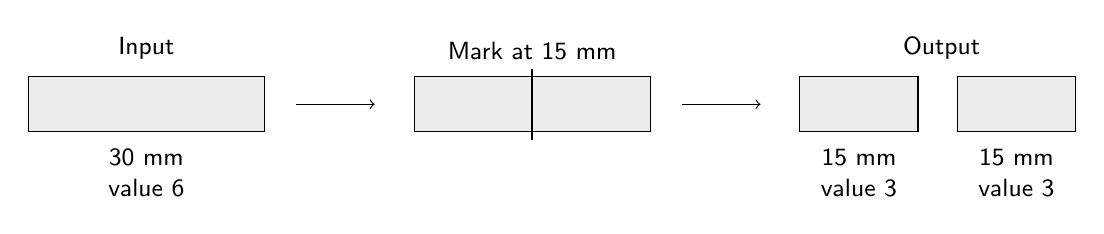
\begin{tikzpicture}[x=1mm,y=1mm,font=\small]
\draw[fill=gray!15] (0,0) rectangle (30,7);
\node[above] at (15,8) {Input};\node[below,align=center] at (15,-1) {30 mm\\value 6};
\draw[->] (34,3.5)--(44,3.5);
\draw[fill=gray!15] (49,0) rectangle (79,7);\draw[thick] (64,-1)--(64,8);
\node[above] at (64,8) {Mark at 15 mm};
\draw[->] (83,3.5)--(93,3.5);
\draw[fill=gray!15] (98,0) rectangle (113,7);\draw[fill=gray!15] (118,0) rectangle (133,7);
\node[above] at (116,8) {Output};
\node[below,align=center] at (105.5,-1) {15 mm\\value 3};
\node[below,align=center] at (125.5,-1) {15 mm\\value 3};
\end{tikzpicture}
\end{center}
Use scrap for this unprinted neutral panel. Read the panel game's first-round example at its table later; do not launch all investigations at once.

\textbf{Adult key notation.} R is a red circle card, B a blue square card; a vertical bar is a cut \emph{between} cards. With two bars give the middle piece to one tray and the two ends to the other.

\begin{minipage}[t]{.46\linewidth}
\sub{K--1 Problem 1 on student page 1}
\small\ktable
\end{minipage}\hfill
\begin{minipage}[t]{.50\linewidth}
\sub{K--1 Problem 2 on student page 2}
\small\ksecond
\end{minipage}

\textbf{K--1 Problem 1 reasoning.} Each tray needs one red/one blue. The only possible single cut is the middle; it fails in rows 2 and 4. The displayed two-gap answers attain the minimum. All shown minimum positions are unique, apart from swapping trays. \hint{``What must each tray have? Does changing the order in a tray change its counts?''}

\textbf{K--1 Problem 2 reasoning.} Row 3's three reds cannot be paired across trays. In other rows, test the only possible one-gap share (the middle) to prove the minimum. Both ends may sit separately in one tray. \hint{``Can you pair every red with one in the other tray? Could one tray hold two pieces?''}
\newpage
\head{K--1 continuations and Grades 2--3 trains}
\sub{K--1 Problem 3 on student page 3}
A challenge succeeds exactly when the first four cards do \emph{not} contain two reds: the only possible one-gap share splits eight cards four/four. There are 34 such orders out of 70; the other 36 have two reds in their first four.

Record successful partner challenges actually played, not all 34. Seven rows are not a promised answer count. Problem 2 row 5 is one such train; if a maker copies it, ask for a different one. \hint{``If both trays need four cards, which gap could possibly work?''} A later continuation is to share the same challenge with two gaps rather than invent more one-gap failures.

\sub{K--1 Problem 4 on student page 4}
Use the separate $240\times40$ mm strip. Two cuts at \textbf{60 and 180 mm from the red end} work: the middle piece and the two ends each contain 60 mm red and 60 mm blue. One straight-across cut cannot split both colours. These are the unique minimum positions. Children fold or match lengths; an adult measures and cuts their marks. \hint{``Does each tray have half of \emph{each} colour? Which colours would one cut split?''} Do not accept a lengthwise cut: the page says straight across.

\sub{K--1 Problem 5 on student page 5}
\textbf{No shareable train needs three gaps.} Even counts always permit at most two by the overview's window argument. Odd-count trains are impossible and do not answer the question. \hint{``Can this train be shared at all? Can a middle piece match the two ends?''} Let a child demonstrate several hard trains; save the general proof for a ready group.

\sub{Grades 2--3 Problem 1 on student page 1}
These are all six colour orders. Same-colour labels do not matter; reversal counts when it changes the word.
\begin{center}\allfour\end{center}
Completeness: sort by the first red's place: first gives three choices for the other red, second gives two, third gives one; $3+2+1=6$. Eight rows include spare space. \hint{``How could you sort your trains so that you notice a missing one?''} Children can pool records rather than each reproduce a catalogue.
\newpage
\head{Grades 2--3 solutions and the marking game}
\sub{Grades 2--3 Problem 2 on student page 2}
\begin{center}\msecond\end{center}
Row 5 has three blues and is impossible. Otherwise test the middle gap; the table attains each minimum. Row 6 has exactly two minimum choices: gaps after cards $(2,7)$ or $(3,8)$, namely \seq{RR|BRRRB|BBR} and \seq{RRB|RRRBB|BR}. All other displayed shareable rows have one minimum choice. \hint{``If one cut worked, how many cards would be on each side?''}

\sub{Grades 2--3 Problem 3 on student page 3}
The answer is the same 60/180 mm division as K--1 Problem 4. Both people give the middle piece value $3/2+1/2=2$, and the ends together value 2. A single cut exact for A is at 80 mm; B's is at 160 mm, so no single cut is exact for both. Read real lengths from the material strip, not a ruler laid on the schematic student picture. \hint{``Use A's card on both trays, then B's on both. What does half a colour contribute?''} The grades 4--5 Problem 3 solution supplies uniqueness and arbitrary-value reasoning.

\sub{Grades 2--3 Problem 4 on student page 4}
\textbf{No.} Use guide page 1's two-gap window proof after experiments invite an explanation. A finger/scrap window can model it. Twelve printed slots are capacity, not required length; use the ten-card kit and sketch larger inventions. Unsystematic failed searches alone do not prove the bound. \hint{``Could a half-length window have too many reds at both ends of its trip?''}

\sub{Grades 2--3 Problems 5 and 6 on student pages 5 and 6}
Use three-person A/B/C and three trays. Page 5's worked XYZ first round is a rule example; the first task game is \textbf{XZY}. Problem 6 adds \textbf{YXZ and ZYX}. For those three games the actual cuts are at 25 and 75 mm. The first and second takers each get own value 4; the remaining person gets 8. Nobody gets less than 4, but somebody envies in each game. The lookup table on guide page 7 also serves grades 4--5 Problem 5.

\textbf{Run sheet (also grades 4--5 Problem 5).}
\begin{enumerate}\setlength{\itemsep}{0pt}\setlength{\parskip}{0pt}
\item Lay X/Y/Z in the printed order beside the actual-size row.
\item Each recipient uses only their own card and initials their first mark on the row.
\item Referee names the leftmost mark; cut or bracket that prefix into the taker's tray.
\item The other two mark again from the new left end, adding a second initial.
\item Last person takes the rest; each uses their own card to check all three trays.
\end{enumerate}
\textbf{Quarter marks still arise.} Each grades 2--3 game has a second-round non-taker's mark at 112.5 mm: a quarter-panel (12.5 mm) into the last panel, worth 2 of 8. The page's half-panel example does not teach quarters. Adults may scribe; knowing this mark lies past 75 mm suffices to choose the taker.

\hint{``From the \emph{new} left end, what does your own card value? Which card are you using for all three trays?''} If the adult must choose the marks rather than read or record them, redo the page's Y-panel example with a real panel. As a later challenge, ask whether a fair third can coexist with wanting another tray; do not compare different people's own scores as an envy test.
\newpage
\head{Grades 4--5 exact halves and fewest cuts}
\sub{Grades 4--5 Problem 1 on student page 1}
\begin{center}\utable\end{center}
Every train is shareable with unique minimum gaps. Row 4's window is cards 5--9, not centred. For four reds/four blues, one cut works exactly when the first four contain two reds: $\binom42^2=36$ of $\binom84=70$ orders; the other 34 need two. \hint{``Where would the only possible one-cut division be?''}

\sub{Grades 4--5 Problem 2 on student page 2}
\textbf{No even-count two-colour train needs more than two cuts.} Act out guide page 1's proof: shift a half-length window one card, losing/adding at most one red. Complementary end windows force a surplus to become a deficit or hit the target. \hint{``Can a whole-number count jump from too many to too few without passing the target?''} More colours are a different problem, not a counterexample to this theorem.

\sub{Grades 4--5 Problem 3 on student page 2}
\textbf{Exactly two cuts, uniquely at 60 and 180 mm}, up to exchanging trays. If a tray holds fractions $r$ of the red and $b$ of the blue, being exact for both people means
\[
3r+b=2,\qquad r+3b=2.
\]
Subtract to get $r=b$, then $r=b=1/2$. With two genuine cuts and two trays, the middle piece must be in one tray and both end pieces in the other; otherwise a cut could be removed. The middle must contain 60 mm of each colour, forcing the two positions. One cut cannot split both colours; alternatively A's unique one-cut half is 80 mm and B's is 160 mm.

\textbf{Any other numbers on these two-colour cards still work with the same cuts.} Half of each colour contributes $(a+b)/2$ for a card valuing the whole panels at $a,b$. This includes zero values and identical tastes, when one cut may suffice and minima need not be unique. \hint{``Which fraction of each colour would work regardless of its price?''} For varying density, the overview's continuous window still gives a two-cut bound, though these same fixed positions may fail.

\sub{Grades 4--5 Problem 4 on student page 3}
\textbf{Three cuts are necessary and sufficient.} Cut each of X, Y, Z in half: at 25, 75 and 125 mm along the row. Give each tray one half of every panel, so each is worth 6 to all three observers. To see why fewer cannot work, let $x,y,z$ be the fractions in one tray. The conditions are
\[
x+2y=3/2,\qquad y+2z=3/2,\qquad 2x+z=3/2.
\]
Their sum gives $x+y+z=3/2$. Comparing with the first equation gives $y=z$; comparing with the second gives $z=x$. Thus all are $1/2$. Each panel needs an interior cut, so at least three are needed. \hint{``Could a whole panel go to just one tray if each observer still saw a tie?''} On one row, these three cut positions and alternating trays are forced, apart from swapping trays. If the panels are separate pieces, any choice of one half of each panel per tray works.
\newpage
\head{Grades 4--5 marking games and guarantee}
\sub{Grades 4--5 Problem 5 on student page 4}
Use the run sheet on guide page 5. Finish XYZ, then try the other five orders. Every coordinate below is in millimetres from the \emph{original} left end of the $150$ mm row. First cut at the first taker's mark; second cut at the second taker's mark; the last person receives everything after it. For example, XYZ gives C $[0,25]$, A $[25,62.5]$, B $[62.5,150]$.
\begin{center}\small\setlength{\tabcolsep}{4pt}\gametable\end{center}
No selected marks tie. XYZ, YZX and ZXY need a quarter-panel cut; the others cut at half-panel points. Allow children to distribute the six trials across pairs or visits and pool records.

\textbf{Complete observer check.} In each triple below the entries value \emph{A's, B's, C's trays in that order}, using only the named observer's card. ``A to B'' means A strictly prefers B's tray. Equal values do not count as envy.
\begin{center}\small\setlength{\tabcolsep}{5pt}\scoretable\end{center}
Thus nobody gets less than 4. The last person's own value is 11 in XYZ, YZX and ZXY, and 8 in XZY, YXZ and ZYX. The two takers have exactly 4. \hint{``Which row of numbers uses your card throughout? Is your own tray at least as valuable as each other one?''}

\sub{Grades 4--5 Problem 6 on student page 5}
The proof is the marking invariant on guide page 1. Use three spaces labelled ``taken'', ``taken'', ``left'': to the waiting person, each removed piece was worth at most 4, leaving at least $12-4-4=4$. Takers get exactly 4. Enough remains for each next mark.

\textbf{The printed generalization needs a qualification.} ``Whatever values the cards give'' is valid when each person aims at one third of \emph{their own original total}, not the fixed number 4 unless that total remains 12. If all three panels were worth 8 to everyone, total 24, taking value 4 would fall below the required 8. For changed cards, announce the new personal targets before playing. Values must remain nonnegative, additive and divisible with no value stuck at a point; negative values or indivisible positive-value cards invalidate this argument.

For the printed cards, giving A whole Y, B whole Z and C whole X gives everyone 8 and no envy: each sees the other two whole panels as 4 and 0. \textbf{The marking game cannot do that well for all three}, in any order: its first two takers receive exactly 4. A guarantee is a floor, not the best allocation. \hint{``What value does the rule force the first taker to receive? What might that person think of a larger tray left later?''}
\newpage
\head{Grades 4--5 card continuations and sources}
\sub{Grades 4--5 Problem 7 on student page 5}
By two-person card A, three reds and two blues total $3+1+3+1+3=11$. Half is $5.5$. In the printed R1 B1 R3 B2 R2 row, cut halfway through paper R3, \textbf{62.5 mm from the left} of the 125 mm row. Each side has one red, one blue and half a red: $3+1+1.5=5.5$. The red circle names the card; value follows the whole square, not the ink.

\textbf{Neither a gap nor the inside of a blue card can be the half point in any order.} Every whole-card running total is an integer, never 5.5. For a blue of value 1 to straddle 5.5, the preceding cards would have to total 5. The only possibility from these values is one red plus both blues; then no blue remains for the cut. \hint{``What totals can you have just before a blue?''} In rearranged trials mark the answer; use an unmounted replacement of whichever red would be cut, never a sturdy card.

\sub{Grades 4--5 Problem 8 on student page 6}
The marking game makes only two \emph{selected} cuts. A cut at a gap splits no card and a cut inside a card splits just that card. This proves at most two distinct cards are split, even if both lie in one card. Use the same uniform-within-card rule as Problem 7, and target each person's own third.

\textbf{No, cutting only one of the two paper reds cannot suffice.} The total is 2 and each person needs $2/3$. The uncut red must go whole to someone; the other two would need $4/3$ from the remaining red of value 1. Cutting that one card repeatedly does not help. The bound is attained by cutting the first red at $2/3$ of its width and the second at $1/3$ of its width: the three consecutive shares each have value $2/3$. On two touching 25 mm cards the locations are $50/3$ and $100/3$ mm from the left. \hint{``Who receives the uncut card, and what is left for the other two?''}

\sub{Sources and boundaries}
The numerical tasks were checked against the final 5/6/6-page student PDFs, the outline, W58-guide-v4 (especially pp. 1--3, 9) and W58-materials-v3. The checker retains exhaustive finite checks; those do not replace the general proofs.

Ariel D. Procaccia, \emph{Cake Cutting Algorithms}, \S\S13.2--13.3.3 (PDF pp. 1--6), is cited through the base guide's consulted range, not claimed newly reread: \href{https://procaccia.info/wp-content/uploads/2020/03/cakechapter.pdf}{procaccia.info, cakechapter.pdf}. It supports the value model and proportional/envy-free distinction; Selfridge--Conway is not taught here.

\textbf{Outline bibliography, not newly consulted.} A. K. Austin, ``Sharing a cake'', \emph{Mathematical Gazette} 66 (1982), 212--215 (continuous window); C. R. Hobby and J. R. Rice, ``A moment problem in L1 approximation'', \emph{Proc. AMS} 16 (1965), 665--670; C. H. Goldberg and D. B. West, ``Bisection of circle colorings'', \emph{SIAM J. Algebraic Discrete Methods} 6 (1985), 93--106; N. Alon and D. B. West, ``The Borsuk--Ulam theorem and bisection of necklaces'', \emph{Proc. AMS} 98 (1986), 623--628. These support the $k$-cut background; no such general theorem is checked by finite enumeration here. Marking background: H. Steinhaus, ``The problem of fair division'', \emph{Econometrica} 16 (1948), 101--104; L. E. Dubins and E. Spanier, ``How to cut a cake fairly'', \emph{AMM} 68 (1961), 1--17.

\textbf{After use.} Record which problems children chose, where adult reading became adult decision-making, and whether the cutting conventions and observer comparisons were retained. Digital mathematical and page checks do not establish physical readiness or successful classroom use.
\end{document}
